\chapter{Análisis} \label{chap:analisis}

\section{Análisis}

En este capítulo se van a exponer diferentes aspectos relacionados con el diseño e implementación. Concretamente, se realiza un análisis de los usuarios objetivo, comprendiendo sus necesidades, expectativas y limitaciones. Asimismo, también se muestran los modelos de caso de uso, la arquitectura del sistema. Conjuntamente, con los modelos de comportamiento y el modelado de entidades y relaciones. De esta manera, se ofrece una visión clara y estructurada de la solución propuesta.

\subsection{Análisis de Usuarios Objetivo}

El enfoque de la plataforma web está dirigido principalmente a niños entre los 8 y 18 años, siguiendo la metodología de CODELEARN S.L.. Donde la mayoría de los clientes son estudiantes con poco o ningún conocimiento previo de programación. Es por ello que la plataforma está diseñada para ser intuitiva y flexible, en línea con las recomendaciones de Large y Beheshti sobre el diseño de interfaces para niños \cite{large2005}.

Si tenemos en cuenta la brevedad del período de atención de los niños y su desarrollo cognitivo en curso, se deberán evitar tareas extensas o excesivamente complicadas. Las expectativas y necesidades son diversas, pero comúnmente incluyen una interfaz visualmente atractiva, instrucciones claras y una retroalimentación inmediata tal como especifican Duglas Frye y Elliot Soloway \cite{interfacedesign}. Asimismo, se han incorporado elementos de gamificación dentro la plataforma con tal mantener el interés y la motivación de los usuarios. 

Finalmente, la plataforma será accesible; es decir, se podrá acceder desde múltiples dispositivos como ordenadores, tablets y smartphones debido a su diseño \textit{Web Responsive}.

\subsection{Análisis de Requisitos Educativos}

La enseñanza de habilidades de programación dentro de las escuelas está cobrando una gran relevancia \cite{teachingcodingchildren}. Sin embargo, hay una falta de herramientas y enfoques efectivos mucho más allá de herramientas como Scratch \cite{teachingcodingchildren}. Conscientes de esta brecha, este sistema educativo adopta un enfoque fundamentado en evidencia y prácticas académicas sólidas.

Aunque lenguajes como Scratch y Logo son de los más populares para la educación de niños, se ha optado por Python, C++, Java y HTML+CSS+JS. Python es conocido por su simplicidad y legibilidad, lo que facilita el aprendizaje para los principiantes \cite{pears2007}. Además, permite una transición fluida a lenguajes más complejos. C++, Java y HTML+CSS+JS, aunque sujetos a debate sobre su idoneidad para principiantes, son cruciales en la industria y la educación. Su relevancia práctica justifica su presencia \cite{dewarschonberg}.

Al ir más allá de los enfoques basados en bloques como Scratch, se busca que los niños aprendan la programación basada en texto, más cercana a la realidad. Los ejercicios se organizan por competencias específicas, permitiendo un aprendizaje adaptable y progresivo. Alineando el enfoque con los resultados de investigaciones sobre el tema \cite{document2010}. 

Es importante destacar que el sistema se ha diseñado para ser inclusivo, ofreciendo ejercicios de diversa dificultad y con un buen sistema de asistencia. De esta manera, se siguen las directrices recomendadas por Luxton-Reily y Wünsche sobre las características de un buen sistema inteligente para la enseñanza de programación \cite{intelligentturoingprogrammingeducation}, consiguiendo un buen enfoque educativo.

\section{Modelos de Caso de Uso y Escenarios de Uso}

En esta sección se va a hablar de las interacciones usuario-sistema. En primer lugar, se abordará los modelos de caso de uso \ref{fig:caso_uso}. Debido a que nos proporcionan una visión panorámica, resaltando las interacciones posibles y los actores implicados. Es decir, nos ayudará a definir lo que el sistema puede hacer y lo que se espera que haga. Además, también se va a especificar los diferentes escenarios de uso, ya que nos proporcionan una mejor comprensión de las interacciones específicas. Pudiendo observar las verdaderas dinámicas del sistema en acción.

Con esta combinación, se establecen las funcionalidades esperadas del sistema y cómo este responderá ante diferentes situaciones y acciones del usuario. Cabe destacar que los diagramas se han realizado mediante PlantULM \cite{planttext}. 

\subsection{Actores del Sistema}

La interacción de la plataforma se basa en tres tipos de usuarios: estudiantes, profesores y administradores. Es importante destacar que el acceso a la plataforma está restringido a usuarios registrados, ya que se busca asegurar que cada interacción dentro del sistema se realice en un entorno seguro y personalizado.

\paragraph{Estudiantes} Los estudiantes son los principales usuarios. Su objetivo es aprender programación a través de los recursos educativos disponibles. Podrán acceder a ejercicios, leer material didáctico, recibir retroalimentación y consultar sus dudas.

\paragraph{Profesores} Su papel es de facilitador de aprendizaje, y de apoyo emocional a los estudiantes. Corrigen los ejercicios de HTML, debido su complejidad de corrección. Además, de la resolución de dudas. También deben ir comprobando los estudiantes que más ejercicios fallen o estén mucho tiempo sin conectarse, para escribirles un correo con tal de motivarles. 

\paragraph{Administradores} Los administradores tienen el máximo nivel de control. Pueden agregar, consultar y editar todo el contenido didáctico de la plataforma. Además, de poder gestionar los profesores.

\begin{figure}[H]
    \centering
    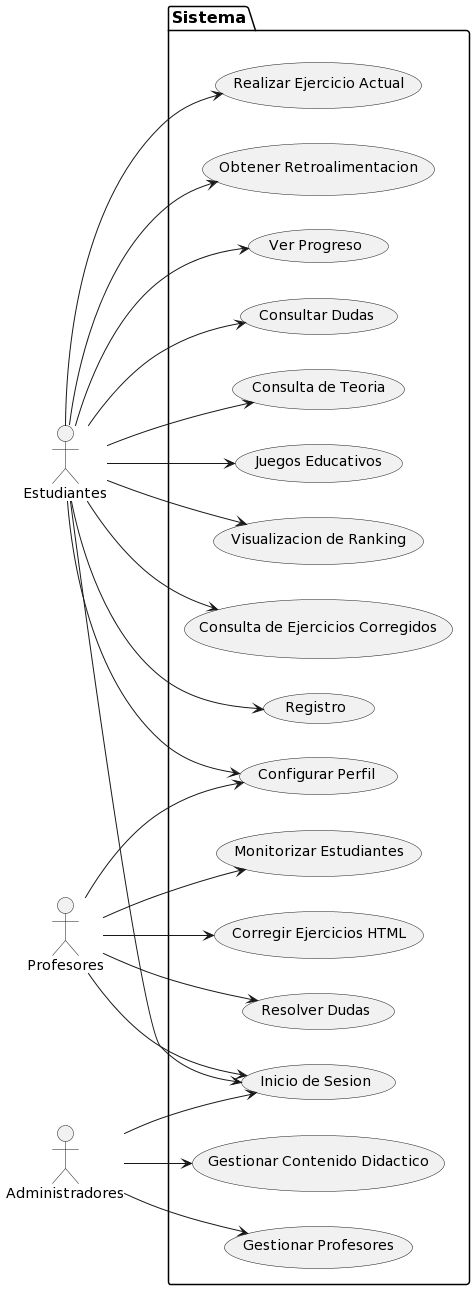
\includegraphics[width=0.3\textwidth]{imagenes/modelo.png}
    \caption{Diagrama de Caso de Uso del sistema}
    \label{fig:caso_uso}
\end{figure}

\subsection{Restricciones y Reglas de Negocio}

Las pautas operativas y limitaciones rigen la interacción de los usuarios con el sistema. Se abordarán las restricciones que afectan a distintos actores y se establecen las reglas que garantizan un entorno seguro y eficiente. Con tal de delinear las condiciones bajo las cuales se opera la plataforma educativa.

\paragraph{Restricciones de Acceso}
\begin{itemize}
    \item Estudiantes: Limitados a módulos y ejercicios asignados por la plataforma.
    \item Profesores: Acceso a corrección de ejercicios HTML y panel de dudas; sin permisos para modificar contenido.
    \item Administradores: Control total en la gestión de contenido y cuentas de profesores.
\end{itemize}

\paragraph{Reglas de Validación}
\begin{itemize}
    \item Los ejercicios tienen un tiempo límite para su realización; de excederlo, se considerarán fallidos.
    \item Puntuación basada en corrección y calidad del código.
    \item Validación manual por profesores para ejercicios HTML.
\end{itemize}

\paragraph{Reglas de Negocio Adicionales}
\begin{itemize}
    \item En caso de fallo en un ejercicio, el estudiante recibe un nuevo problema para evitar la desmotivación.
    \item Los profesores pueden identificar y enviar correos motivacionales a estudiantes con bajo rendimiento o actividad.
    \item Solo administradores pueden añadir o eliminar cuentas de profesores.
\end{itemize}

\subsection{Escenarios de Uso Detallados}

Dentro de esta subsección se ofrece un análisis de los escenarios de uso que involucran a los distintos tipos de usuarios. Concretamente, se va a presentar una serie de tablas que detallarán cada escenario de uso.

A continuación, se describen los elementos que compondrán cada tabla de escenarios de uso, siguiendo las pautas sugeridas por expertos en usabilidad:

\begin{itemize}
    \item \textbf{ID}: Código de identificación único para cada escenario de uso.
    \item \textbf{Nombre}: Título descriptivo.
    \item \textbf{Actor}: Define los usuarios que están implicados en la acción.
    \item \textbf{Descripción}: Una breve explicación del escenario de uso. 
    \item \textbf{Precondiciones}: Condiciones o eventos que deben cumplirse o suceder antes de que se inicie el escenario de uso.
    \item \textbf{Postcondición}: Resultados o estados que se alcanzan después de completar el escenario de uso.
    \item \textbf{Flujo}: Detalla todos los pasos implicados para la realización de cada caso de uso, incluyendo tanto el flujo básico como cualquier flujo alternativo.
\end{itemize}

Los escenarios están centrados en los factores más interesantes de la plataforma diseñada. Es importante destacar que se ha decidido omitir los casos de uso tales como inicio de sesión, registro o cerrar sesión con tal de evitar la redundancia debido a su lógica común. 

\begin{table}[H]
    \centering
    \begin{tabularx}{\textwidth}{|l|X|}
    \hline
    ID & EU-1 \\
    \hline
    Nombre & Realización de un ejercicio \\
    \hline
    Actor & Estudiante \\
    \hline
    Descripción & El estudiante resuelve un ejercicio de programación. \\
    \hline
    Precondiciones & Estudiante ha iniciado sesión y no ha completado todos los módulos. \\
    \hline
    Postcondición & El ejercicio se marca como completado y el estudiante recibe retroalimentación. \\
    \hline
    Flujo & 
    1. Accede al módulo que aún no tenga completado. \\
    & 2. Se le abre un ejercicio. \\
    & 3. Resuelve el ejercicio dentro del tiempo límite. \\
    & 4. Envía la solución. \\
    & 5. Recibe retroalimentación y puntuación si es pertinente. \\
    \hline
    \end{tabularx}
    \caption{EU-1: Realización de un ejercicio}
\end{table}

\begin{table}[H]
    \centering
    \begin{tabularx}{0.9\textwidth}{|l|X|}
    \hline
    ID & EU-2 \\
    \hline
    Nombre & Tiempo superado en un ejercicio \\
    \hline
    Actor & Estudiante \\
    \hline
    Descripción & El estudiante no logra completar un ejercicio de programación dentro del tiempo límite. \\
    \hline
    Precondiciones & Estudiante ha iniciado sesión y está resolviendo un ejercicio. \\
    \hline
    Postcondición & El ejercicio se marca como erróneo y se le muestra un nuevo ejercicio. \\
    \hline
    Flujo & 
    1. El estudiante está resolviendo un ejercicio. \\
    & 2. El tiempo límite se alcanza antes de que el estudiante envíe la solución. \\
    & 3. El ejercicio se marca como fallado. \\
    & 4. Se le presenta un nuevo ejercicio al estudiante. \\
    \hline
    \end{tabularx}
    \caption{EU-2: Tiempo superado en un ejercicio}
\end{table}

\begin{table}[H]
    \centering
    \begin{tabularx}{\textwidth}{|l|X|}
    \hline
    ID & EU-3\\
    \hline
    Nombre & Corrección de ejercicios por parte del profesor \\
    \hline
    Actor & Profesor \\
    \hline
    Descripción & El profesor corrige manualmente ejercicios HTML debido a su complejidad. \\
    \hline
    Precondiciones & Profesor ha iniciado sesión, y algún estudiante ha enviado un ejercicio de HTML para corrección. \\
    \hline
    Postcondición & Ejercicio corregido y retroalimentación enviada al estudiante. \\
    \hline
    Flujo & 
    1. Inicia sesión en la plataforma. \\
    & 2. Accede a la lista de ejercicios HTML pendientes de corrección. \\
    & 3. Selecciona un ejercicio para corregir. \\
    & 4. Evalúa el ejercicio y escribe una retroalimentación. \\
    & 5. Envía los datos y se marca el ejercicio como corregido. \\
    \hline
    \end{tabularx}
    \caption{EU-3: Corrección de ejercicios por parte del profesor}
\end{table}

\begin{table}[H]
    \centering
    \begin{tabularx}{\textwidth}{|l|X|}
    \hline
    ID & EU-4 \\
    \hline
    Nombre & Administrador gestionando contenido didáctico \\
    \hline
    Actor & Administrador \\
    \hline
    Descripción & El administrador añade, edita o elimina contenido educativo en la plataforma. \\
    \hline
    Precondiciones & Administrador ha iniciado sesión. \\
    \hline
    Postcondición & Contenido educativo actualizado en la plataforma. \\
    \hline
    Flujo & 
    1. Inicia sesión en la plataforma. \\
    & 2. Accede al panel de administración de contenido didáctico. \\
    & 3. Selecciona la opción para añadir, editar o eliminar según el tipo de contenido. \\
    & 4. Realiza las acciones correspondientes. \\
    & 5. Confirma los cambios. \\
    \hline
    \end{tabularx}
    \caption{EU-4: Gestión del contenido didáctico}
\end{table}

\begin{table}[H]
    \centering
    \begin{tabularx}{\textwidth}{|l|X|}
    \hline
    ID & EU-5 \\
    \hline
    Nombre & Resolución de dudas \\
    \hline
    Actor & Estudiante, Profesor \\
    \hline
    Descripción & El estudiante plantea una duda y el profesor la resuelve. \\
    \hline
    Precondiciones & Estudiante y profesor han iniciado sesión. \\
    \hline
    Postcondición & Duda resuelta. \\
    \hline
    Flujo & 
    1. Estudiante accede a la sección de dudas. \\
    & 2. Escribe y envía su pregunta. \\
    & 3. Profesor visualiza en el panel la duda. \\
    & 4. Accede a la duda. \\
    & 5. Resuelve la duda proporcionando una explicación detallada. \\
    & 6. Estudiante recibe notificación de que su esta duda resuelta. \\
    \hline
    \end{tabularx}
    \caption{EU-5: Resolución de dudas}
\end{table}

\subsection{Seguridad y Acceso}

Para garantizar la integridad de la plataforma, es crucial abordar aspectos de seguridad y acceso.

\paragraph{Autenticación}
La plataforma adopta un sistema de autenticación. Esto se logra mediante el uso de correo electrónico y contraseña. 

\paragraph{Autorización}
Los roles de usuario, es decir, estudiantes, profesores y administradores, vienen con diferentes niveles de acceso. Los profesores, por ejemplo, pueden corregir ejercicios y resolver dudas, pero no tienen permisos para alterar el contenido didáctico.

\paragraph{Seguridad de Datos}
La seguridad de los datos es una prioridad. Por ello, todas las transmisiones de datos se realizan mediante conexiones HTTPS seguras. Además, técnicas de hash y salting modernas aseguran que las contraseñas se almacenen de manera segura.

\paragraph{Monitorización y Auditoría}
Finalmente, mantenemos un registro de todas las actividades significativas en la plataforma. Esto permite a los administradores realizar un seguimiento detallado y, si es necesario, controlar las actividades de los usuarios.

\section{Arquitectura del Sistema}

La interacción del usuario en el Frontend se lleva a cabo utilizando tecnologías estándar como HTML sin emplear \textit{frameworks} adicionales para su desarrollo. Además, la interfaz es \textit{Web Responsive}, lo que garantiza su adaptación a variados dispositivos. Desde el punto de vista de la seguridad, se han implementado medidas como la validación de entradas, previniendo así amenazas como los ataques XSS. Los datos de sesión se conservan en el cliente mediante cookies.

Por otro lado, el Backend se ha desarrollado con Flask. Se encarga de administrar las API RESTful y de establecer una conexión ininterrumpida con la base de datos PostgreSQL. La biblioteca \textit{flask\_login} respalda las funcionalidades de autenticación y autorización, aportando una capa de seguridad adicional. La lógica de negocio del sistema reside principalmente en el Sistema de Tutoría Inteligente (ITS). Este subsistema es el encargado de la elección y evaluación de ejercicios, ofreciendo retroalimentación y monitoreando el avance del estudiante.

En relación con la seguridad del Backend, se han establecido roles y restricciones de acceso coherentes con las reglas de negocio previamente determinadas. Aunque la arquitectura actual no posee herramientas concretas orientadas a la escalabilidad, está concebida para ser resistente y estable.

Es esencial destacar que, la estructura general del sistema sigue el patrón Modelo-Vista-Controlador (MVC). La Vista reside en el Frontend, y el Controlador y Nodelo en el Backend \ref{fig:arqsistema}. Este patrón facilita la distinción entre la lógica de la interfaz de usuario y las operaciones, simplificando su mantenimiento.

\begin{figure}[H]
    \centering
    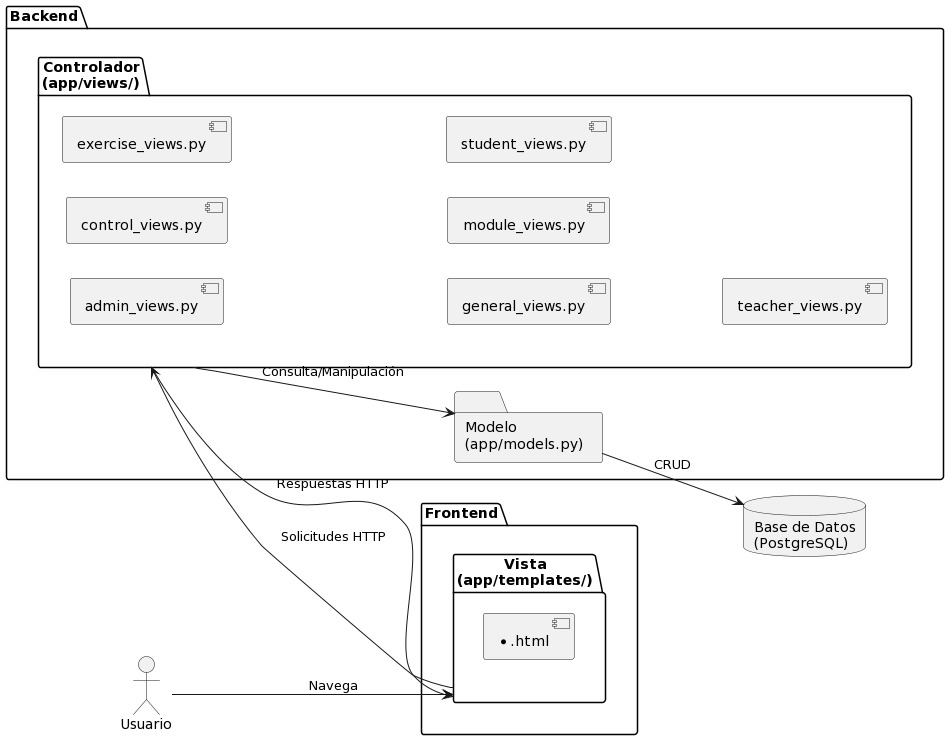
\includegraphics[width=\textwidth]{imagenes/ArquitecturaDeSistema.jpeg}
    
    \caption{Arquitectura de sistema}
    \label{fig:arqsistema}
\end{figure}

\section{Modelos de Comportamiento}

\subsection{Diagrama de Corrección y Evaluación de calidad del código}

El verdadero reto comienza tras la entrega de un ejercicio por parte del estudiante. La lógica de corrección evalúa el código en términos de precisión y calidad. Si un código no alcanza un estándar mínimo, el sistema propone ejercicios adicionales, reforzando así las áreas de mejora del estudiante \ref{fig:correccion}. La justificación detrás de esta lógica se centra en la premisa de que la repetición y el refuerzo son esenciales para consolidar el aprendizaje. Además, al establecer estándares de calidad, se fomentan las buenas prácticas de programación desde las etapas iniciales de formación.

\begin{figure}[H]
    \centering
    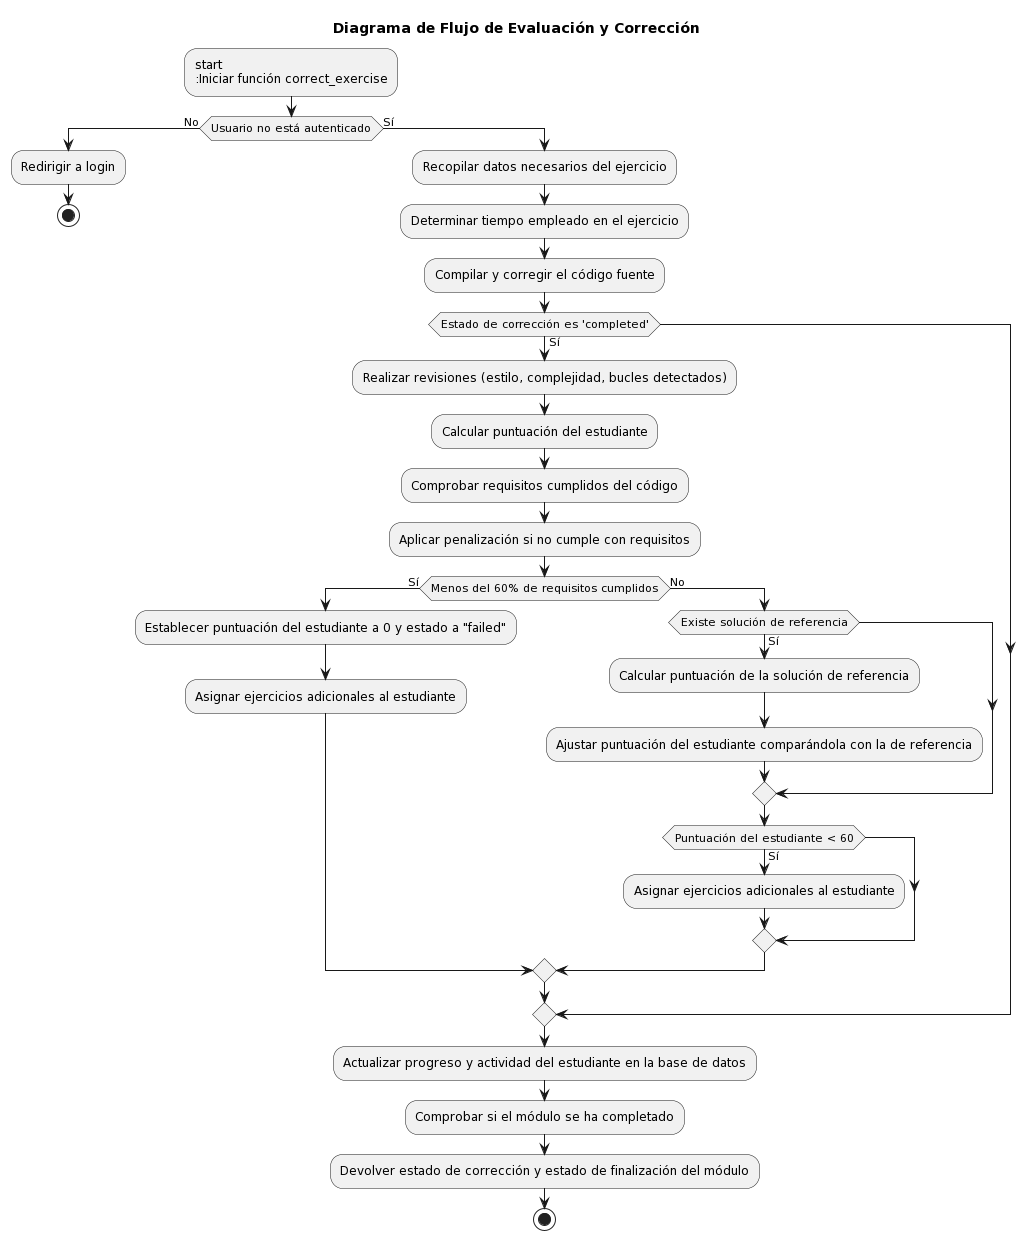
\includegraphics[width=\textwidth]{imagenes/correcionejercicios.png}
    
    \caption{Diagrama de flujo para la corrección del código}
    \label{fig:correccion}
\end{figure}

\subsection{Diagrama para la Selección y Evaluación de ejercicios}

El sistema prioriza la progresión estructurada del estudiante. Al ingresar, la plataforma identifica ejercicios en curso o determina el próximo paso en función de los requisitos del módulo. Esta estructura garantiza que, antes de enfrentarse a cualquier tarea, los conceptos teóricos relevantes sean presentados al estudiante \ref{fig:seleccion}. Esta estrategia se fundamenta en la pedagogía moderna, que sugiere que la teoría y la práctica deben ir de la mano para un aprendizaje óptimo.

\begin{figure}[H]
\centering
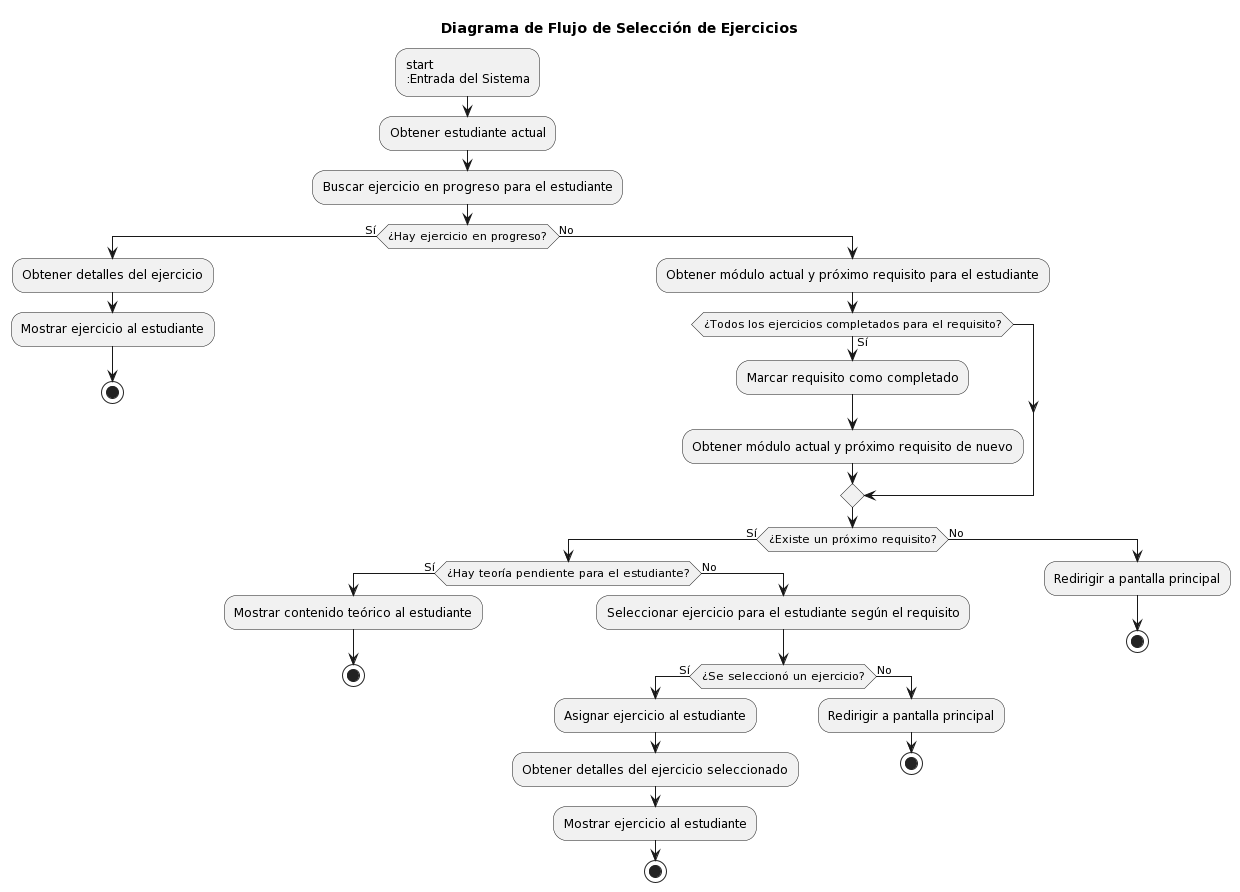
\includegraphics[width=\textwidth]{imagenes/seleccionejercicios.png}
\caption{Diagrama de flujo para la selección de ejercicios}
\label{fig:seleccion}
\end{figure}


\section{Modelado de Entidades y sus Relaciones}

En este apartado se va a hablar sobre el modelado de datos, que es esencial para comprender la estructura y las relaciones entre las distintas entidades en una base de datos. Este proyecto gira alrededor de la gestión educativa. Aquí, usuarios como estudiantes y administradores interactúan con módulos, ejercicios, teorías y otros componentes. Las relaciones entre estas entidades garantizan una coherencia y eficiencia en el sistema. 

El Diagrama Entidad-Relación (ER) \ref{fig:erdiagram} es la representación gráfica. Muestra entidades como tablas y sus interconexiones mediante líneas. Las cardinalidades en las relaciones aportan información sobre cómo interactúan estas entidades.

Este diagrama desvela varias entidades clave: Users, Exercises, Theory y Modules. Las conexiones entre ellas reflejan la lógica de negocio y los requisitos del sistema. Por ejemplo, un usuario puede tener en progreso varios ejercicios. Sin embargo, cada progreso es único para un usuario. En paralelo, un módulo puede albergar múltiples ejercicios y teorías. Aun así, cada uno pertenece solo a un módulo.


\newpage

\begin{figure}[H]
    \centering
    \begin{sideways}
        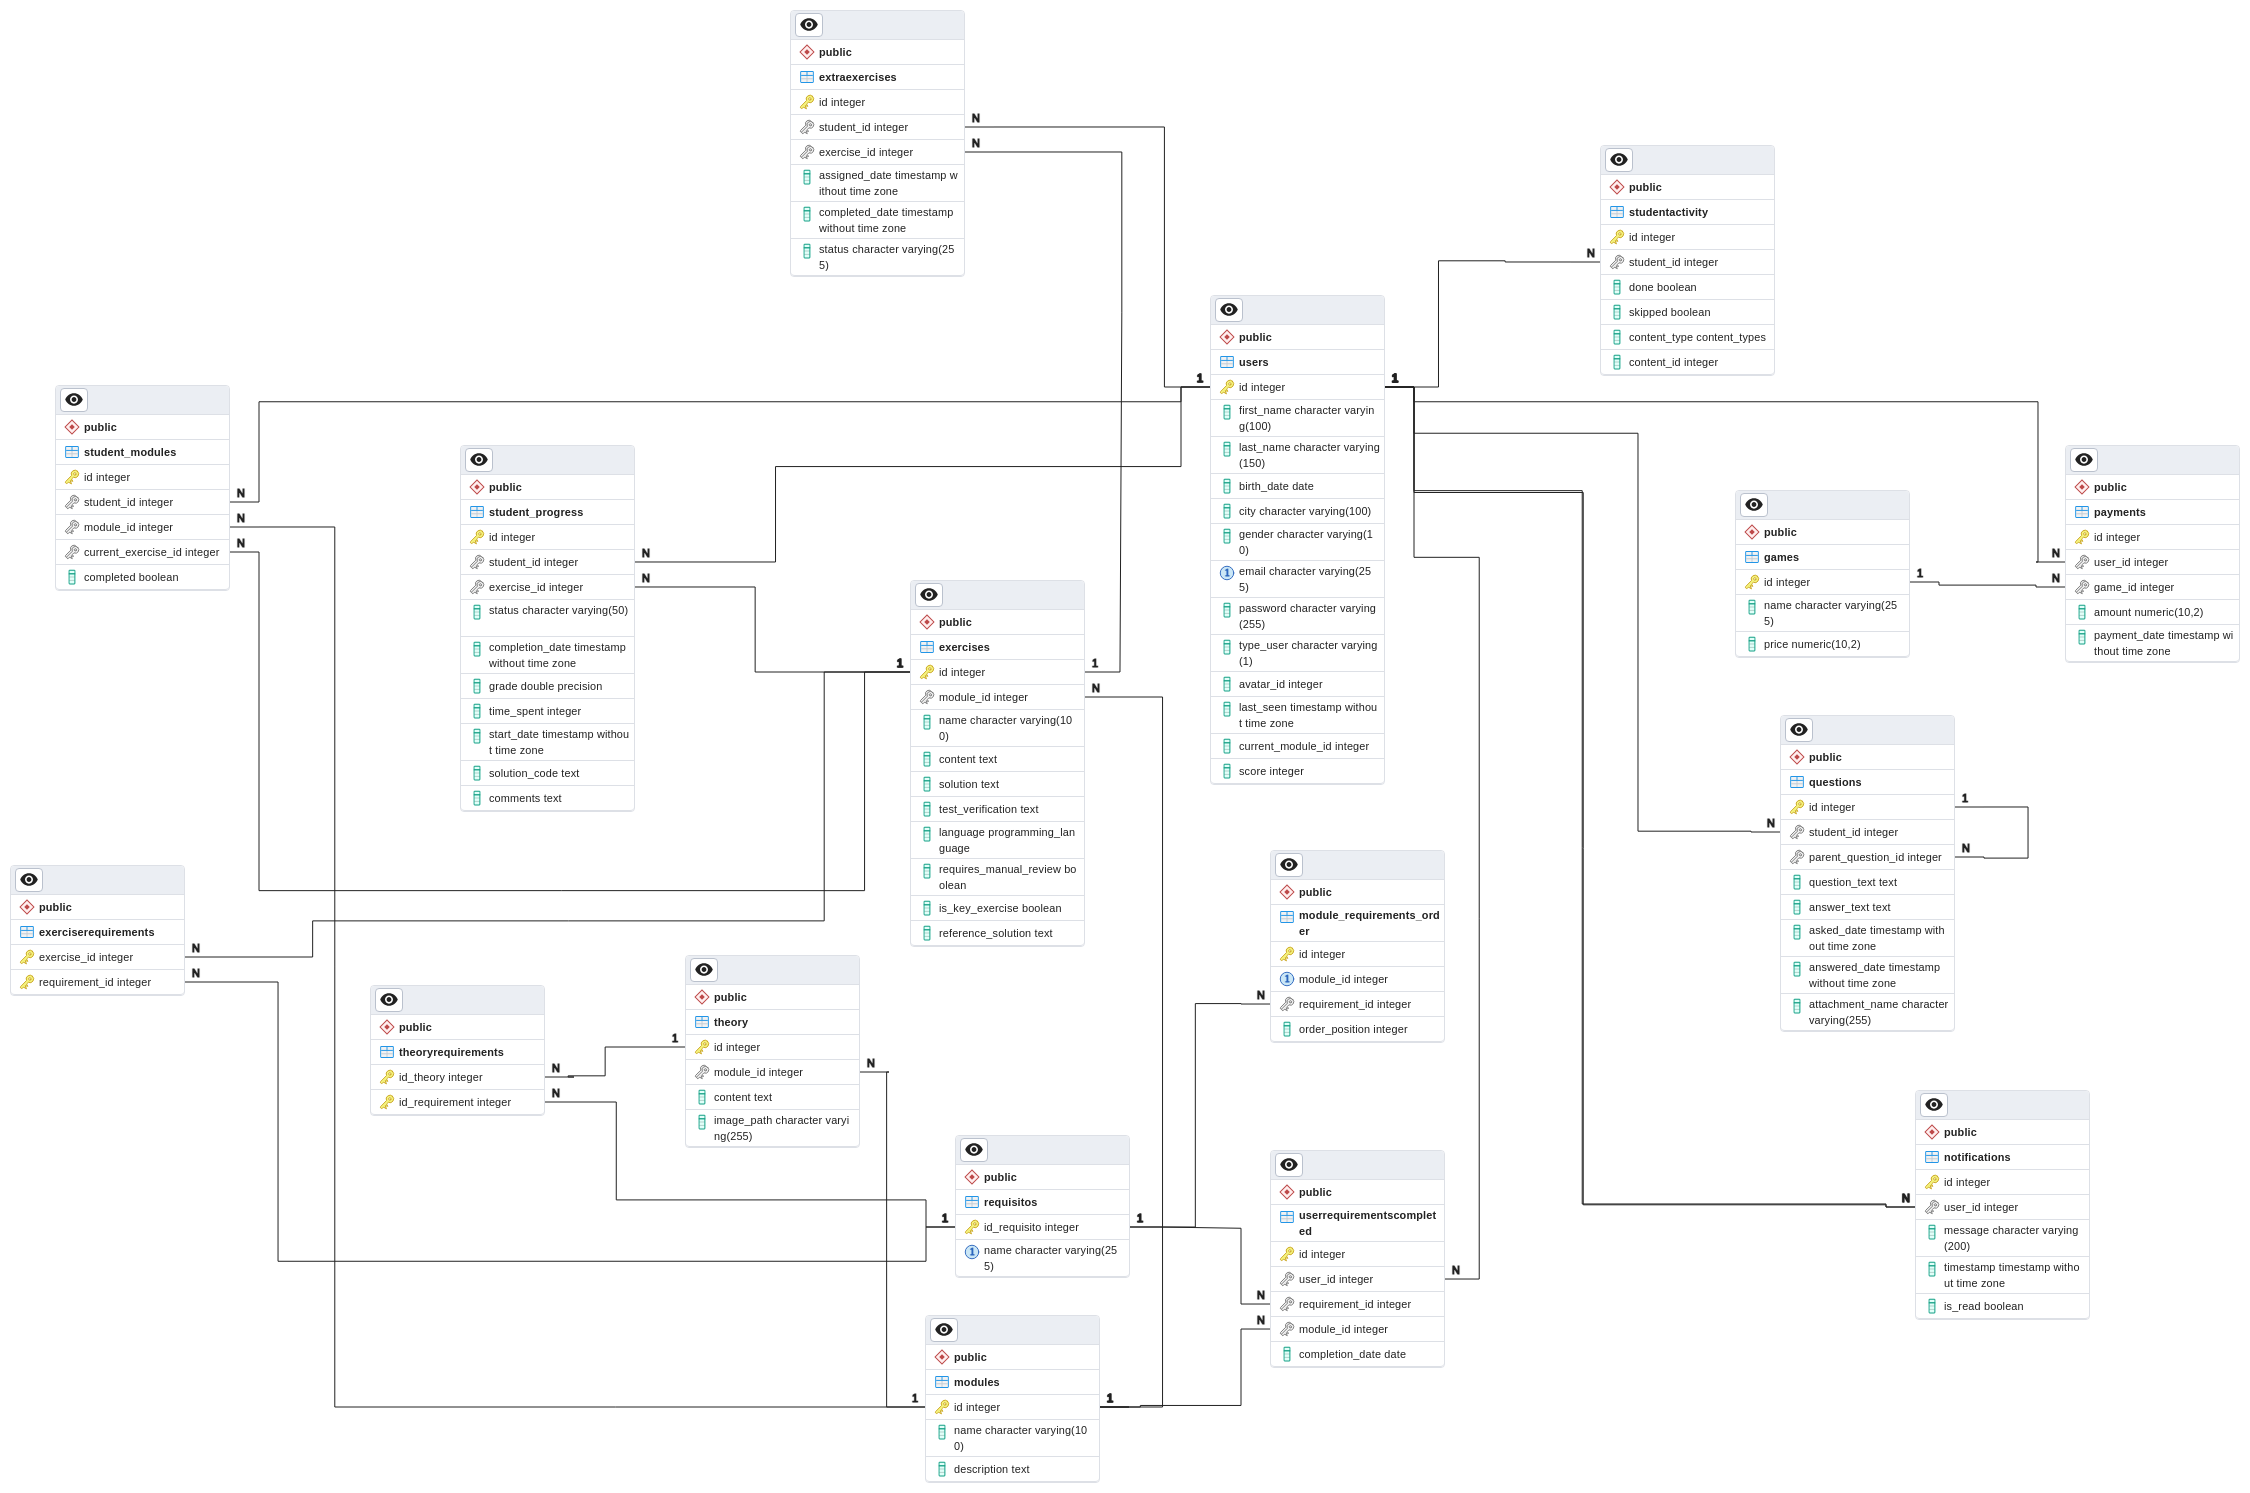
\includegraphics[width=1.8\textwidth]{imagenes/er.png}
    \end{sideways}
    \caption{Diagrama Entidad-Relación}
    \label{fig:erdiagram}
\end{figure}